\documentclass[10pt,twocolumn]{article}

% ---------- Geometry & core packages ----------
\usepackage[margin=0.75in,columnsep=22pt]{geometry}
\usepackage[table]{xcolor}
\usepackage{amsmath}
\usepackage{amssymb}
\usepackage{array}
\usepackage{booktabs}
\usepackage{tabularx}
\usepackage{caption}
\usepackage{enumitem}
\usepackage{titlesec}
\usepackage{fancyhdr}
\usepackage{tikz}
\usetikzlibrary{positioning,calc,arrows.meta}
\usepackage[most]{tcolorbox}
\usepackage{fontawesome5}
\usepackage[hidelinks]{hyperref}

% ---------- Palette ----------
\definecolor{deepteal}{RGB}{0,77,89}
\definecolor{coral}{RGB}{224,110,79}
\definecolor{slate}{RGB}{51,58,64}
\definecolor{mist}{RGB}{236,242,243}

\hypersetup{colorlinks=true, linkcolor=deepteal, citecolor=deepteal, urlcolor=coral}

% ---------- Section styling ----------
\titleformat{\section}
  {\color{deepteal}\large\bfseries}
  {\thesection}{0.6em}{}
  [{\color{coral}\vspace{-0.9em}\titlerule[1.1pt]}]
\titlespacing*{\section}{0pt}{1.1em}{0.6em}

\titleformat{\subsection}
  {\color{slate}\bfseries\itshape}
  {\thesubsection}{0.5em}{}
\titlespacing*{\subsection}{0pt}{0.8em}{0.3em}

% ---------- Header / footer ----------
\pagestyle{fancy}
\fancyhf{}
\renewcommand{\headrulewidth}{0pt}
\renewcommand{\footrulewidth}{0.4pt}
\fancyfoot[L]{\footnotesize\color{slate!70}MIS 2026 \textbar\ Track C: Data, Environment \& Society}
\fancyfoot[R]{\footnotesize\color{slate!70}\thepage}

% ---------- Custom commands ----------
\newcommand{\affmark}[1]{\textsuperscript{#1}}

\newtcolorbox{contribbox}{
  colback=mist, colframe=deepteal, boxrule=0.6pt,
  arc=2pt, left=6pt, right=6pt, top=5pt, bottom=5pt,
  title={\faLightbulb\ \textbf{Key Contributions}}, fonttitle=\color{white}\bfseries,
  colbacktitle=deepteal, coltitle=white,
  fontupper=\small
}

\newtcolorbox{policybox}{
  colback=white, colframe=coral, boxrule=0.7pt,
  arc=2pt, left=6pt, right=6pt, top=5pt, bottom=5pt,
  title={\faBalanceScale\ \textbf{Policy Recommendation}}, fonttitle=\color{white}\bfseries,
  colbacktitle=coral, coltitle=white,
  fontupper=\small
}

\newtcolorbox{notebox}{
  colback=mist, colframe=slate, boxrule=0.4pt,
  arc=1pt, left=6pt, right=6pt, top=5pt, bottom=5pt,
  fontupper=\small\itshape
}

\setlength{\parindent}{0pt}
\setlength{\parskip}{4pt}

\begin{document}

% =====================================================================
% FULL-WIDTH TITLE BLOCK
% =====================================================================
\makeatletter
\twocolumn[{%
\begin{@twocolumnfalse}

\begin{flushright}

\begin{tikzpicture}
\node[fill=deepteal, text=white, rounded corners=3pt, inner sep=5pt, font=\small\bfseries]
  {Track C \textbar\ Data, Environment \& Society};
\end{tikzpicture}
\end{flushright}

\vspace{-0.3cm}
{\footnotesize\color{coral}\bfseries \faCalendar\ Meridian Interdisciplinary Symposium (MIS 2026) \quad \textbar\quad Short Paper Track}

\vspace{0.35cm}
{\color{deepteal}\Huge\bfseries Reading the City's Fever: A Cross-Disciplinary Sensor Mesh for Urban Heat Island Detection\par}

\vspace{0.45cm}

\noindent
\begin{minipage}[t]{0.32\textwidth}
\centering
\textbf{Elena Cho}\affmark{1}\\
\small Dept.\ of Environmental Engineering\\
Vertex Institute of Technology\\
\href{mailto:e.cho@vertex.edu}{\faEnvelope\ e.cho@vertex.edu}
\end{minipage}\hfill
\begin{minipage}[t]{0.32\textwidth}
\centering
\textbf{Marcus Reyes}\affmark{2}\\
\small Dept.\ of Public Policy\\
Nimbus University\\
\href{mailto:m.reyes@nimbus.edu}{\faEnvelope\ m.reyes@nimbus.edu}
\end{minipage}\hfill
\begin{minipage}[t]{0.32\textwidth}
\centering
\textbf{Priya Nair}\affmark{3}\\
\small Dept.\ of Computer Science\\
Apex Polytechnic\\
\href{mailto:p.nair@apex.edu}{\faEnvelope\ p.nair@apex.edu}
\end{minipage}

\vspace{0.5cm}

\begin{tcolorbox}[colback=mist, colframe=deepteal, boxrule=0.7pt, arc=2pt,
  left=8pt, right=8pt, top=6pt, bottom=6pt]
\textbf{\color{deepteal}Abstract.}\ Urban heat islands (UHIs) are typically studied either through
sparse fixed-station meteorology or through remote-sensing imagery that misses fine-grained,
street-level variation. This paper reports on a nine-month deployment of a low-cost, solar-powered
sensor mesh across four neighborhoods of the fictional city of Meridian Bay, combined with a
lightweight edge-to-cloud pipeline and a policy-facing dashboard co-designed with municipal
planners. We show that intra-neighborhood temperature differentials reach $3.8^\circ$C on
summer afternoons, that tree-canopy fraction is the strongest single predictor of cooling, and
that translating raw sensor output into planning-relevant tiers required iterative input from
environmental engineers, computer scientists, and policy analysts working as a single team
rather than in sequence. We argue that this three-way loop, not the sensor hardware itself, is
the paper's main contribution, and we offer a template for symposium tracks that bring these
communities together.
\vspace{2pt}\\
\textbf{Keywords:} urban heat islands, low-cost sensing, edge computing, interdisciplinary
methods, environmental policy
\end{tcolorbox}

\vspace{0.35cm}

\begin{contribbox}
\begin{itemize}[leftmargin=1.1em, itemsep=1pt, topsep=2pt]
  \item A 42-node solar sensor mesh built from off-the-shelf components, validated against two
    reference-grade weather stations ($R^2 = 0.94$).
  \item An edge-aggregation pipeline that reduces uplink volume by 87\% without discarding
    peak-hour resolution.
  \item A four-tier confidence scoring scheme that lets non-technical planners read sensor
    output without a statistics background.
  \item A reflection on where three-discipline collaboration broke down and what fixed it,
    offered as a working note for other symposium tracks.
\end{itemize}
\end{contribbox}

\vspace{0.4cm}
\end{@twocolumnfalse}
}]
\makeatother
\thispagestyle{empty}

% =====================================================================
% BODY
% =====================================================================

\section{Introduction}
Cities warm unevenly. A parking lot and a shaded park three blocks apart can differ by several
degrees at the same hour, yet the instruments that most municipal climate offices rely on --
one or two airport-grade weather stations -- cannot see that difference at all. Remote sensing
fills part of the gap, but satellite thermal bands report surface temperature, not the air
temperature that determines whether a resident on a heat-advisory day is actually at risk.

The Meridian Bay Urban Resilience Office asked our three groups -- an environmental engineering
lab, a public policy program, and a computer science department -- to jointly answer a
deceptively simple question: \emph{which blocks need cooling infrastructure first, and how
confident should the answer be?} Answering it required a sensor network cheap enough to deploy
at block-level density, a computing pipeline that could turn a firehose of noisy readings into
something stable, and a policy framing that a city council member could act on inside a single
meeting. No one discipline could deliver all three.

This short paper documents the resulting system and, more importantly, the collaboration
pattern that made it work. Section~2 situates the work relative to existing UHI literature.
Section~3 describes the sensor mesh and data pipeline. Section~4 reports measured
temperature differentials and model performance. Section~5 turns to the interdisciplinary
process itself and the policy tiers it produced. Section~6 concludes with limitations and a
proposed second deployment.

\section{Related Work}

\subsection{Environmental sensing approaches}
Fixed reference stations remain the gold standard for accuracy but are far too sparse for
intra-neighborhood analysis; a typical mid-sized city operates fewer than five. Satellite
land-surface-temperature products offer full coverage but at 30--100\,m resolution and with
a systematic offset from near-surface air temperature that varies by land cover, making them
unreliable for block-by-block ranking.

\subsection{Low-cost sensor meshes}
Citizen-science temperature networks have grown considerably, but most published deployments
report raw readings without an explicit confidence model, leaving planners to decide, on their
own, how much to trust a single noisy node. Prior edge-computing work on environmental sensor
networks has focused on power efficiency and uplink cost, treating the choice of what to report
to end users as an implementation detail rather than a design question in its own right.

\subsection{Interdisciplinary translation}
A recurring theme in the policy-informatics literature is that technically sound analysis
frequently fails to change municipal decisions because it is delivered in a form decision-makers
cannot act on under time pressure. Few empirical reports describe \emph{how} the translation
step was actually built, which is the gap this paper tries to fill.

\section{Methodology}

\subsection{Sensor mesh design}
We deployed 42 solar-powered nodes across four neighborhoods chosen to span a land-use gradient:
dense commercial core, mixed residential, light industrial, and a tree-lined residential edge
adjacent to Fen Hollow Park. Each node combines a shielded temperature/humidity probe, a
low-power microcontroller, and a mesh radio, reporting every six minutes to the nearest of six
gateway nodes.

\subsection{Edge-to-cloud pipeline}
Raw six-minute readings are noisy and expensive to transmit continuously, so gateways perform a
local rolling-median filter and only forward a reading when it deviates from the filtered
baseline by more than $0.3^\circ$C, or every 30 minutes regardless, whichever comes first. This
single rule cut uplink volume by 87\% while preserving the sharp transitions that occur at dawn
and at sunset, which turned out to be the intervals planners cared about most. Figure~\ref{fig:pipeline}
summarizes the resulting architecture.

\begin{figure}[t]
\centering
\begin{tikzpicture}[
  node distance=8mm and 6mm,
  box/.style={draw=deepteal, fill=mist, rounded corners=3pt, minimum width=2.5cm,
    minimum height=0.85cm, align=center, font=\footnotesize},
  lbl/.style={font=\scriptsize\itshape, color=slate}
]
\node[box] (mesh) {\faLeaf\ Sensor Mesh\\42 nodes};
\node[box, below=of mesh] (gw) {\faWifi\ Edge Gateways\\rolling-median filter};
\node[box, below=of gw] (cloud) {\faCloud\ Cloud Aggregator\\4-tier scoring};
\node[box, below=of cloud] (dash) {\faChartBar\ Planning Dashboard};

\draw[-{Latex[length=2mm]}, deepteal] (mesh) -- (gw);
\draw[-{Latex[length=2mm]}, deepteal] (gw) -- (cloud);
\draw[-{Latex[length=2mm]}, deepteal] (cloud) -- (dash);

\node[lbl, right=2mm of mesh] {Environmental Eng.};
\node[lbl, right=2mm of gw] {Computer Science};
\node[lbl, right=2mm of cloud] {Computer Science};
\node[lbl, right=2mm of dash] {Public Policy};
\end{tikzpicture}
\caption{Edge-to-cloud pipeline, annotated by the discipline that owned each stage.}
\label{fig:pipeline}
\end{figure}

\subsection{Confidence tiers}
Sensor uptime varied node to node, so raw averages could quietly hide a neighborhood with three
working sensors behind one with fifteen. We assign each neighborhood-hour a confidence tier
(High/Medium/Low/Insufficient) from active node count, agreement between neighboring nodes, and
distance to the nearest reference station, and we surface only the tier -- not the underlying
statistics -- on the planning dashboard.

\section{Results}
Table~\ref{tab:results} reports mean afternoon temperature differential ($\Delta T$, relative to
the airport reference station) by neighborhood over the nine-month deployment window
(March--November).

\begin{table*}[t]
\centering
\caption{Neighborhood-level summer-afternoon temperature differential and mesh confidence.}
\label{tab:results}
\begin{tabularx}{\textwidth}{X l c c c}
\toprule
\textbf{Neighborhood} & \textbf{Dominant land use} & \textbf{Mean $\Delta T$ ($^\circ$C)} & \textbf{Active sensors} & \textbf{Confidence tier} \\
\midrule
\rowcolor{mist} Harborview Core & Dense commercial & $+3.8$ & 11 & High \\
Cedar Row & Mixed residential & $+2.1$ & 12 & High \\
\rowcolor{mist} Ironworks District & Light industrial & $+3.1$ & 9 & Medium \\
Fen Hollow Edge & Residential, tree canopy & $+0.4$ & 10 & High \\
\bottomrule
\end{tabularx}
\end{table*}

Tree-canopy fraction was the single strongest predictor of afternoon cooling in a simple linear
model ($\beta = -0.41$, $p < 0.01$), ahead of albedo proxies and building density, echoing
smaller-scale canopy studies but at a spatial grain those studies could not resolve. Harborview
Core, with under 8\% canopy cover, ran nearly $3.4^\circ$C hotter on average than Fen Hollow Edge
at the same hour, on the same day, under the same synoptic weather.

\section{Cross-Disciplinary Implications}
The technical results in Section~4 were not, in practice, the hard part. The hard part was
agreeing on what a "reading" meant to each group at the table.

\begin{notebox}
Early in the project, the environmental engineers wanted raw $\Delta T$ values with full
uncertainty bars; the computer scientists wanted to report only what the pipeline could
validate automatically; the policy team wanted a single traffic-light indicator per block.
None of these, alone, was usable by the other two groups. The four-tier confidence label in
Section~3.3 is the artifact that resulted from resolving that disagreement, not from any one
discipline's preferred format.
\end{notebox}

Once the tier system was in place, the policy team could rank neighborhoods for a pilot
cooling-infrastructure budget without needing to interpret a confidence interval, while the
engineering and computing teams retained the full underlying data for their own analysis. We
believe this pattern -- a shared, deliberately lossy summary layer sitting on top of a full
technical record -- generalizes past this specific project.

\begin{policybox}
Based on the High-confidence tiers, we recommend the Urban Resilience Office prioritize
Harborview Core for the first tranche of reflective-surface and street-tree pilots, with
Ironworks District as the second phase once additional sensor coverage raises it out of the
Medium tier.
\end{policybox}

\section{Conclusion and Future Work}
A 42-node solar sensor mesh, an edge-filtering pipeline, and a four-tier confidence scheme let a
three-discipline team turn noisy street-level temperature data into a ranked, actionable list for
a real cooling-infrastructure budget. The technical pieces are unremarkable in isolation; the
contribution is the shared summary layer that let each discipline keep its own rigor while still
producing one artifact the others could use.

Limitations remain: nine months covers only one growing season, gateway coverage in Ironworks
District was thinner than planned, and the confidence-tier thresholds were tuned on this
deployment and not yet validated elsewhere. A second deployment, planned for spring 2027, will
add two more neighborhoods and test whether the tier thresholds transfer without re-tuning.

\section*{Acknowledgments}
{\small We thank the Meridian Bay Urban Resilience Office for pilot-site access, and Vertex
Institute of Technology's Environmental Engineering workshop for sensor-housing fabrication.}

\begin{thebibliography}{9}
\small
\bibitem{oke} T.~Oke-style, ``Boundary-layer processes and canopy heat retention in mid-sized
  cities,'' \emph{Journal of Urban Climate Studies}, vol.~14, no.~2, pp.~112--130, 2019.
\bibitem{alvarez} R.~Alvarez and T.~Kessler, ``Distributed microclimate sensing for urban
  canopy studies,'' in \emph{Proc.\ Intl.\ Conf.\ on Environmental Sensing}, 2021, pp.~55--63.
\bibitem{nimbus-policy} M.~Reyes, ``From dashboards to decisions: translating environmental
  data for municipal budgets,'' \emph{Policy Informatics Review}, vol.~7, pp.~201--219, 2022.
\bibitem{edge-sensing} P.~Nair and D.~Okonkwo, ``Rolling-median edge filtering for low-power
  environmental telemetry,'' in \emph{Proc.\ ACM Conf.\ on Embedded Sensing Systems}, 2020,
  pp.~301--310.
\bibitem{canopy} S.~Whitfield, ``Canopy fraction as a predictor of near-surface cooling: a
  meta-analysis,'' \emph{Landscape and Urban Planning}, vol.~198, 2020.
\bibitem{citizen-sci} L.~Bergstrom, ``Citizen sensor networks for climate adaptation
  planning,'' \emph{Environmental Data Science}, vol.~3, no.~1, pp.~1--18, 2021.
\bibitem{remote-sensing} J.~Park and H.~Adeyemi, ``Limits of satellite land-surface
  temperature for block-level heat assessment,'' \emph{Remote Sensing of Environment},
  vol.~256, 2021.
\bibitem{interdisciplinary} C.~Marchetti, ``Boundary objects in interdisciplinary science
  teams,'' \emph{Science, Technology \& Human Values}, vol.~45, no.~4, pp.~610--633, 2020.
\end{thebibliography}

\end{document}
